% REALBIM architecture (Fig. 3). Build: xelatex fig1_framework.tex (next to fig1_icons.tex).
% (a) producer, the BIM layer (slot pool and borrow bits), recipients R1-R4;
% (b) a zoom into recipient R1: the ReadSeal layer (sealed plan offline, check and enroll online).
% Numbered steps follow frame k: admit, commit and send, accept/check/enroll, return, reuse, deliver.
% Text is set in Carlito (metric-compatible with the Calibri of Figs. 2-6). Icons: Lucide (ISC) and
% Tabler (MIT) outline icons converted to TikZ paths by svg2tikz.py; see ICONS-LICENSE.txt.
\documentclass[border=0pt]{standalone}
\usepackage{fontspec}
\setmainfont{Carlito}
\usepackage{tikz}
\usepackage{pifont}
\usetikzlibrary{arrows.meta,calc,patterns}
% Generated by svg2tikz.py from Lucide (ISC) and Tabler (MIT) icons; see ICONS-LICENSE.txt.
\expandafter\def\csname ico@Lcamera\endcsname{\draw (13.997,4) .. controls (14.732,4) and (15.408,4.403) .. (15.757,5.05) -- (16.243,5.95) .. controls (16.592,6.597) and (17.268,7) .. (18.003,7) -- (20,7) .. controls (21.105,7) and (22,7.895) .. (22,9) -- (22,18) .. controls (22,19.105) and (21.105,20) .. (20,20) -- (4,20) .. controls (2.895,20) and (2,19.105) .. (2,18) -- (2,9) .. controls (2,7.895) and (2.895,7) .. (4,7) -- (5.997,7) .. controls (6.731,7) and (7.406,6.598) .. (7.756,5.952) -- (8.245,5.048) .. controls (8.595,4.402) and (9.27,4) .. (10.004,4) -- cycle; \draw (12,13) circle (3);}
\expandafter\def\csname ico@Lradar\endcsname{\draw (19.07,4.93) .. controls (15.868,1.725) and (10.912,1.073) .. (6.99,3.34); \fill (4,6) circle (1); \draw (2.29,9.62) .. controls (1.261,13.811) and (3.037,18.19) .. (6.695,20.48) .. controls (10.353,22.77) and (15.067,22.455) .. (18.388,19.699) .. controls (21.709,16.943) and (22.887,12.367) .. (21.31,8.35); \draw (16.24,7.76) .. controls (14.672,6.183) and (12.36,5.602) .. (10.233,6.252) .. controls (8.106,6.901) and (6.513,8.673) .. (6.093,10.857) .. controls (5.673,13.041) and (6.495,15.278) .. (8.23,16.67); \fill (12,18) circle (1); \draw (17.99,11.66) .. controls (18.1,13.59) and (17.274,15.455) .. (15.77,16.67); \draw (12,12) circle (2); \draw (13.41,10.59) -- (19.07,4.93);}
\expandafter\def\csname ico@Lgpu\endcsname{\draw (2,17) -- (20,17) .. controls (21.105,17) and (22,16.105) .. (22,15) -- (22,7) .. controls (22,5.895) and (21.105,5) .. (20,5) -- (2,5); \draw (2,21) -- (2,3); \draw (7,17) -- (7,20) .. controls (7,20.552) and (7.448,21) .. (8,21) -- (13,21) .. controls (13.552,21) and (14,20.552) .. (14,20) -- (14,17); \draw (16,11) circle (2); \draw (8,11) circle (2);}
\expandafter\def\csname ico@Lfilter\endcsname{\draw (10,20) .. controls (10,20.379) and (10.214,20.726) .. (10.553,20.895) -- (12.553,21.895) .. controls (12.863,22.05) and (13.231,22.033) .. (13.526,21.851) .. controls (13.821,21.669) and (14,21.347) .. (14,21) -- (14,14) .. controls (14,13.504) and (14.184,13.027) .. (14.517,12.659) -- (21.74,4.67) .. controls (22.004,4.377) and (22.072,3.956) .. (21.912,3.595) .. controls (21.752,3.234) and (21.395,3.001) .. (21,3) -- (3,3) .. controls (2.605,3) and (2.247,3.233) .. (2.087,3.594) .. controls (1.926,3.955) and (1.993,4.377) .. (2.258,4.67) -- (9.483,12.659) .. controls (9.816,13.027) and (10,13.504) .. (10,14) -- cycle;}
\expandafter\def\csname ico@Lusers\endcsname{\draw (16,21) -- (16,19) .. controls (16,16.791) and (14.209,15) .. (12,15) -- (6,15) .. controls (3.791,15) and (2,16.791) .. (2,19) -- (2,21); \draw (16,3.128) .. controls (17.764,3.585) and (18.996,5.177) .. (18.996,7) .. controls (18.996,8.823) and (17.764,10.415) .. (16,10.872); \draw (22,21) -- (22,19) .. controls (21.999,17.177) and (20.765,15.586) .. (19,15.13); \draw (9,7) circle (4);}
\expandafter\def\csname ico@Lfingerprint\endcsname{\draw (12,10) .. controls (10.895,10) and (10,10.895) .. (10,12) .. controls (10,13.02) and (9.9,14.51) .. (9.74,16); \draw (14,13.12) .. controls (14,15.5) and (14,19.5) .. (13,22); \draw (17.29,21.02) .. controls (17.41,20.42) and (17.72,18.72) .. (17.79,18); \draw (2,12) .. controls (2,7.696) and (4.754,3.874) .. (8.838,2.513) .. controls (12.921,1.152) and (17.417,2.557) .. (20,6); \fill (2,16) circle (1); \draw (21.8,16) .. controls (22,14) and (21.931,10.646) .. (21.8,10); \draw (5,19.5) .. controls (5.5,18) and (6,15) .. (6,12) .. controls (5.999,11.319) and (6.114,10.643) .. (6.34,10); \draw (8.65,22) .. controls (8.86,21.34) and (9.1,20.68) .. (9.22,20); \draw (9,6.8) .. controls (10.857,5.728) and (13.145,5.728) .. (15.002,6.801) .. controls (16.858,7.874) and (18.001,9.856) .. (18,12) -- (18,14);}
\expandafter\def\csname ico@Lstamp\endcsname{\draw (14,13) -- (14,8.5) .. controls (14,7) and (15,7) .. (15,5) .. controls (15,3.343) and (13.657,2) .. (12,2) .. controls (10.343,2) and (9,3.343) .. (9,5) .. controls (9,7) and (10,7) .. (10,8.5) -- (10,13); \draw (20,15.5) .. controls (20,14.119) and (18.881,13) .. (17.5,13) -- (6.5,13) .. controls (5.119,13) and (4,14.119) .. (4,15.5) -- (4,17) .. controls (4,17.552) and (4.448,18) .. (5,18) -- (19,18) .. controls (19.552,18) and (20,17.552) .. (20,17) -- cycle; \draw (5,22) -- (19,22);}
\expandafter\def\csname ico@Linbox\endcsname{\draw (22,12) -- (16,12) -- (14,15) -- (10,15) -- (8,12) -- (2,12); \draw (5.45,5.11) -- (2,12) -- (2,18) .. controls (2,19.105) and (2.895,20) .. (4,20) -- (20,20) .. controls (21.105,20) and (22,19.105) .. (22,18) -- (22,12) -- (18.55,5.11) .. controls (18.212,4.43) and (17.519,4) .. (16.76,4) -- (7.24,4) .. controls (6.481,4) and (5.788,4.43) .. (5.45,5.11) -- cycle;}
\expandafter\def\csname ico@Tobjectscan\endcsname{\draw (8,10) .. controls (8,8.895) and (8.895,8) .. (10,8) -- (14,8) .. controls (15.105,8) and (16,8.895) .. (16,10) -- (16,14) .. controls (16,15.105) and (15.105,16) .. (14,16) -- (10,16) .. controls (8.895,16) and (8,15.105) .. (8,14) -- (8,10); \draw (3,7) -- (3,5) .. controls (3,3.895) and (3.895,3) .. (5,3) -- (7,3); \draw (3,17) -- (3,19) .. controls (3,20.105) and (3.895,21) .. (5,21) -- (7,21); \draw (17,3) -- (19,3) .. controls (20.105,3) and (21,3.895) .. (21,5) -- (21,7); \draw (17,21) -- (19,21) .. controls (20.105,21) and (21,20.105) .. (21,19) -- (21,17);}
\expandafter\def\csname ico@Lcrosshair\endcsname{\draw (12,12) circle (10); \draw (22,12) -- (18,12); \draw (6,12) -- (2,12); \draw (12,6) -- (12,2); \draw (12,22) -- (12,18);}
\expandafter\def\csname ico@Lroute\endcsname{\draw (6,19) circle (3); \draw (9,19) -- (17.5,19) .. controls (19.433,19) and (21,17.433) .. (21,15.5) .. controls (21,13.567) and (19.433,12) .. (17.5,12) -- (6.5,12) .. controls (4.567,12) and (3,10.433) .. (3,8.5) .. controls (3,6.567) and (4.567,5) .. (6.5,5) -- (15,5); \draw (18,5) circle (3);}
\expandafter\def\csname ico@Ldatabase\endcsname{\draw (12,5) ellipse (9 and 3); \draw (3,5) -- (3,19) .. controls (3,20.657) and (7.029,22) .. (12,22) .. controls (16.971,22) and (21,20.657) .. (21,19) -- (21,5); \draw (3,12) .. controls (3,13.657) and (7.029,15) .. (12,15) .. controls (16.971,15) and (21,13.657) .. (21,12);}
\expandafter\def\csname ico@Lrefreshcw\endcsname{\draw (3,12) .. controls (3,7.029) and (7.029,3) .. (12,3) .. controls (14.516,3.009) and (16.931,3.991) .. (18.74,5.74) -- (21,8); \draw (21,3) -- (21,8) -- (16,8); \draw (21,12) .. controls (21,16.971) and (16.971,21) .. (12,21) .. controls (9.484,20.991) and (7.069,20.009) .. (5.26,18.26) -- (3,16); \draw (8,16) -- (3,16) -- (3,21);}


% muted palette, same hues as the plots (blue = BIM / after return, green = borrow held, amber = frame)
\definecolor{ink}{HTML}{1F2933}\definecolor{sub}{HTML}{5F6B7A}\definecolor{line}{HTML}{9AA5B1}
\definecolor{faint}{HTML}{D9DEE4}\definecolor{paper}{HTML}{F5F7FA}\definecolor{hdr}{HTML}{E8ECF1}
\definecolor{bimD}{HTML}{1F4E8C}\definecolor{bimA}{HTML}{3A73C0}\definecolor{bimT}{HTML}{DCE7F6}\definecolor{bimF}{HTML}{EFF4FB}
\definecolor{rsD}{HTML}{2E6B34}\definecolor{rsA}{HTML}{5AA05F}\definecolor{rsT}{HTML}{DDEEDB}\definecolor{rsF}{HTML}{F2F8F1}
\definecolor{frD}{HTML}{B07A12}\definecolor{frA}{HTML}{E9B23A}\definecolor{frT}{HTML}{F8E3AE}\definecolor{frF}{HTML}{FFF6DF}
\definecolor{pvD}{HTML}{3A73C0}\definecolor{pvT}{HTML}{DCE7F6}
\definecolor{coral}{HTML}{C8414B}

\newcommand{\fs}[1]{\fontsize{#1}{#1}\selectfont}
\newcommand{\var}[1]{\textit{#1}}
\newdimen\icou
\newcommand{\icon}[4][]{% \icon[<style>]{<name>}{<center>}{<size pt>}
  \icou=\dimexpr #4pt/24\relax
  \begin{scope}[shift={#3},x=\icou,y=-\icou,shift={(-12,-12)},line width=1.8\icou,
                line cap=round,line join=round,#1]
    \csname ico@#2\endcsname
  \end{scope}}
\newcommand{\step}[2]{\node[circle,fill=ink,text=white,inner sep=0pt,minimum size=8.4pt,
  font=\fs{6.5}\bfseries] at (#1) {#2};}
% a 3D tensor block: \tensor[<ghost>]{center}{w}{h}
\newcommand{\tensor}[4][]{%
  \begin{scope}[shift={#2}]
    \pgfmathsetmacro{\w}{#3/2}\pgfmathsetmacro{\h}{#4/2}\def\d{3.4}
    \ifx&#1&
      \fill[frT,draw=frD,line width=.45pt] (-\w,\h) -- (-\w+\d,\h+\d) -- (\w+\d,\h+\d) -- (\w,\h) -- cycle;
      \fill[frA,draw=frD,line width=.45pt] (\w,-\h) -- (\w+\d,-\h+\d) -- (\w+\d,\h+\d) -- (\w,\h) -- cycle;
      \fill[frF,draw=frD,line width=.5pt] (-\w,-\h) rectangle (\w,\h);
      \foreach \i in {1,2,3}{\draw[frD!45,line width=.25pt] ({-\w+\i*#3/4},-\h) -- ({-\w+\i*#3/4},\h);}
      \foreach \i in {1,2}{\draw[frD!45,line width=.25pt] (-\w,{-\h+\i*#4/3}) -- (\w,{-\h+\i*#4/3});}
    \else
      \draw[line,line width=.45pt,dash pattern=on 1.4pt off 1.1pt] (-\w,\h) -- (-\w+\d,\h+\d) -- (\w+\d,\h+\d) -- (\w+\d,-\h+\d) -- (\w,-\h);
      \draw[line,line width=.45pt,dash pattern=on 1.4pt off 1.1pt,fill=white] (-\w,-\h) rectangle (\w,\h);
      \draw[line,line width=.45pt,dash pattern=on 1.4pt off 1.1pt] (\w,\h) -- (\w+\d,\h+\d);
    \fi
  \end{scope}}
% a process window: \win{x0}{y0}{x1}{y1}{title}{border}
\newcommand{\win}[6]{%
  \fill[white,rounded corners=3pt] (#1,#2) rectangle (#3,#4);
  \fill[hdr,rounded corners=3pt] (#1,#4-9) rectangle (#3,#4);
  \fill[hdr] (#1,#4-9) rectangle (#3,#4-5);
  \draw[#6,line width=.6pt,rounded corners=3pt] (#1,#2) rectangle (#3,#4);
  \foreach \i/\c in {0/coral,1/frA,2/rsA}{\fill[\c] (#1+4.5+\i*3.6,#4-4.5) circle (1.15);}
  \node[font=\fs{6.9}\bfseries,anchor=west,inner sep=0pt] at (#1+15,#4-4.6) {#5};}

\begin{document}
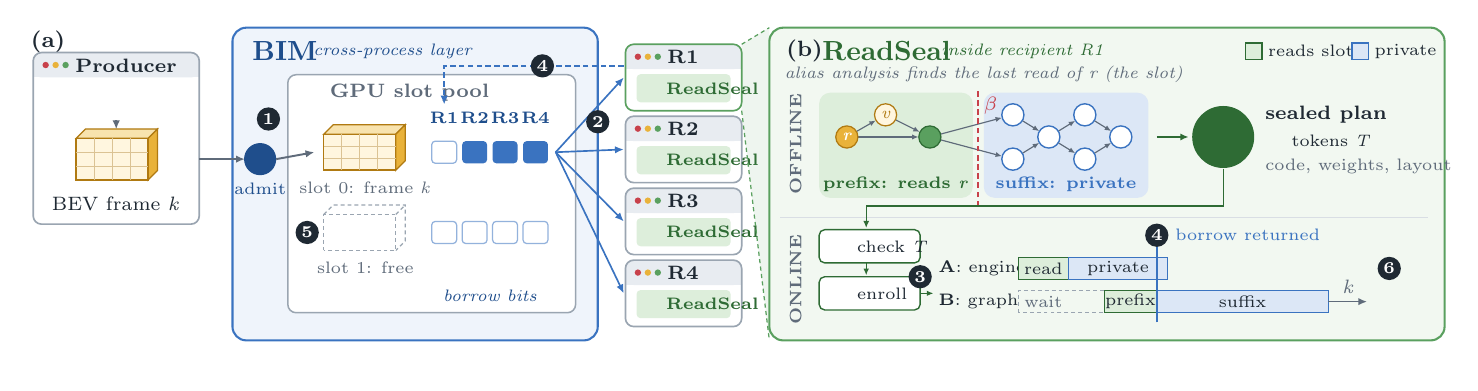
\begin{tikzpicture}[x=1pt,y=1pt,font=\fs{6.8},text=ink,
  data/.style={-{Latex[length=3.2pt,width=2.7pt]},line width=.7pt,draw=sub},
  ctrl/.style={-{Latex[length=3.2pt,width=2.7pt]},line width=.7pt,draw=bimA},
  lbl/.style={font=\fs{6.4},text=sub,inner sep=0pt},
]
\useasboundingbox (0,0) rectangle (514,121);

% =====================================================================
% (a) producer, BIM, recipients
% =====================================================================
\node[font=\fs{7.6}\bfseries,anchor=west,inner sep=0pt] at (1,116) {(a)};

% ---- producer ----
\win{2}{50}{62}{112}{Producer}{line}
\icon[draw=sub]{Lcamera}{(20,95)}{10.5}
\icon[draw=sub]{Lradar}{(44,95)}{10.5}
\draw[data,line width=.55pt] (32,87.5) -- (32,84.3);
\tensor{(30.5,73.5)}{26}{15}
\node[font=\fs{6.6}] at (32,57.5) {BEV frame \var{k}};

% ---- BIM: the slot pool and the borrow bits ----
\draw[bimA,line width=.75pt,fill=bimF,rounded corners=5pt] (74,8) rectangle (206,121);
\node[font=\fs{10}\bfseries,text=bimD,anchor=west,inner sep=0pt] at (81,112.5) {BIM};
\node[font=\fs{6.5}\itshape,text=bimD,anchor=west,inner sep=0pt] at (103,112.5) {cross-process layer};
% GPU memory with two slots; one bit per recipient beside each slot
\draw[line,line width=.55pt,fill=white,rounded corners=3pt] (94,18) rectangle (198,104);
\icon[draw=sub]{Lgpu}{(102.5,97.5)}{8.5}
\node[font=\fs{6.6}\bfseries,text=sub,anchor=west,inner sep=0pt] at (109,97.5) {GPU slot pool};
\foreach \c in {1,...,4}{\node[font=\fs{6}\bfseries,text=bimD] at ({150.5+(\c-1)*11},88.5) {R\c};}
\node[font=\fs{6}\itshape,text=bimD] at (167,24) {borrow bits};
\foreach \y/\lab in {76/{slot 0: frame \var{k}},47/{slot 1: free}}{
  \node[lbl,anchor=north] at (122,\y-10.5) {\lab};}
\tensor{(120,76)}{26}{13}
\tensor[ghost]{(120,47)}{26}{13}
\foreach \y/\c in {76/1,47/1,47/2,47/3,47/4}{
  \draw[bimA!55,line width=.45pt,fill=white,rounded corners=1.3pt] ({146+(\c-1)*11},\y-4) rectangle ++(9,8);}
\foreach \c in {2,3,4}{\fill[bimA,rounded corners=1.3pt] ({146+(\c-1)*11},72) rectangle ++(9,8);}
% admission gate on the way in
\draw[data] (62,73.5) -- (78.5,73.5);
\filldraw[bimD] (84,73.5) circle (5.6);
\icon[draw=white,line width=1.3pt]{Lfilter}{(84,73.1)}{7}
\node[font=\fs{6.2},text=bimD] at (84,62.8) {admit};
\draw[data] (89.8,73.5) -- (103.6,76);
\step{87,88}{1}
% slot reuse once every bit is clear
\icon[draw=bimA]{Lrefreshcw}{(141,47)}{8}
\step{101,47}{5}

% ---- recipients R1-R4, each with ReadSeal inside ----
\foreach \r/\y/\ic in {1/91/Tobjectscan,2/65/Lcrosshair,3/39/Lroute,4/13/Ldatabase}{
  \ifnum\r=1 \def\bc{rsA}\else\def\bc{line}\fi
  \win{216}{\y}{258}{\y+24}{R\r}{\bc}
  \icon[draw=sub]{\ic}{(250,\y+19.5)}{7.2}
  \fill[rsT,rounded corners=1.5pt] (220,\y+3) rectangle (254,\y+13.2);
  \icon[draw=rsD]{Lstamp}{(226,\y+8.1)}{7.5}
  \node[font=\fs{6}\bfseries,text=rsD,anchor=west,inner sep=0pt] at (230.5,\y+8.1) {ReadSeal};}
% (2) commit: bits are set, then descriptors (k, s) fan out to every recipient
\foreach \y in {103,77,51,25}{\draw[ctrl,line width=.6pt] (190.8,76) -- (215.4,\y);}
\step{206,87}{2}

% (4) R1 returns its borrow: its bit is cleared
\draw[ctrl,dash pattern=on 2pt off 1.2pt] (215.4,107.2) -- (150.5,107.2) -- (150.5,93.2);
\step{186,107.2}{4}

% ---- zoom into R1 ----
\fill[rsA,opacity=.10] (258,115) -- (268,121) -- (268,8) -- (258,91) -- cycle;
\draw[rsA,line width=.45pt,dash pattern=on 1.5pt off 1.2pt] (258,115) -- (268,121);
\draw[rsA,line width=.45pt,dash pattern=on 1.5pt off 1.2pt] (258,91) -- (268,8);

% =====================================================================
% (b) ReadSeal inside recipient R1
% =====================================================================
\draw[rsA,line width=.75pt,fill=rsF,rounded corners=5pt] (268,8) rectangle (512,121);
\node[font=\fs{7.6}\bfseries,anchor=west,inner sep=0pt] at (274,112.5) {(b)};
\node[font=\fs{10}\bfseries,text=rsD,anchor=west,inner sep=0pt] at (287,112.5) {ReadSeal};
\node[font=\fs{6.5}\itshape,text=rsD,anchor=west,inner sep=0pt] at (330,112.5) {inside recipient R1};
% color key, shared by the graph and the reader bars
\draw[rsD,fill=rsT,line width=.45pt] (440,109.5) rectangle ++(6,6);
\node[font=\fs{6.2},anchor=west,inner sep=0pt] at (448,112.5) {reads slot};
\draw[pvD,fill=pvT,line width=.45pt] (478.5,109.5) rectangle ++(6,6);
\node[font=\fs{6.2},anchor=west,inner sep=0pt] at (486.5,112.5) {private};
% phase labels
\node[font=\fs{6.4}\bfseries,text=sub,rotate=90] at (277.5,79) {OFFLINE};
\node[font=\fs{6.4}\bfseries,text=sub,rotate=90] at (277.5,30) {ONLINE};
\draw[faint,line width=.5pt] (272,52.5) -- (506,52.5);

% ---- offline: analyze the graph once per model version, seal the plan ----
\fill[rsT,rounded corners=4pt] (286,59.5) rectangle (341.5,97.5);
\fill[pvT,rounded corners=4pt] (345.5,59.5) rectangle (405,97.5);
\node[font=\fs{6.3}\bfseries,text=rsD] at (313.7,64.5) {prefix: reads \var{r}};
\node[font=\fs{6.3}\bfseries,text=pvD] at (375.2,64.5) {suffix: private};
\coordinate (r) at (296,81.5);\coordinate (v) at (310,89.5);\coordinate (a) at (326,81.5);
\coordinate (b1) at (356,89.5);\coordinate (b2) at (356,73.5);\coordinate (b3) at (369,81.5);
\coordinate (b4) at (382,89.5);\coordinate (b5) at (382,73.5);\coordinate (b6) at (395,81.5);
\foreach \a/\b in {r/v,v/a,r/a,a/b1,a/b2,b1/b3,b2/b3,b3/b4,b3/b5,b4/b6,b5/b6}{
  \draw[-{Latex[length=2.3pt,width=1.9pt]},sub,line width=.42pt,shorten >=4.1pt,shorten <=4.1pt] (\a) -- (\b);}
\filldraw[frD,fill=frA,line width=.45pt] (r) circle (4);
\node[font=\fs{5.8}\bfseries\itshape,text=white] at (r) {r};
\filldraw[frD,fill=frF,line width=.45pt] (v) circle (4);
\node[font=\fs{5.6}\itshape,text=frD] at (v) {v};
\filldraw[rsD,fill=rsA,line width=.45pt] (a) circle (4);
\foreach \n in {b1,b2,b3,b4,b5,b6}{\filldraw[pvD,fill=white,line width=.5pt] (\n) circle (4);}
\draw[coral,line width=.75pt,dash pattern=on 2pt off 1.3pt] (343.5,56.5) -- (343.5,99);
\node[font=\fs{7.4}\itshape,text=coral] at (348,92.8) {$\beta$};
\node[font=\fs{6.2}\itshape,text=sub] at (345.5,104.1) {alias analysis finds the last read of \var{r} (the slot)};
% the seal: the plan is bound to the code, weights, and input layout it was built for
\draw[-{Latex[length=3pt,width=2.6pt]},rsD,line width=.6pt] (408,81.5) -- (419.5,81.5);
\filldraw[rsD] (432,81.5) circle (11);
\icon[draw=white,line width=1.5pt]{Lstamp}{(432,82)}{13}
\node[font=\fs{6.9}\bfseries,anchor=west,inner sep=0pt] at (447,89.5) {sealed plan};
\icon[draw=rsD]{Lfingerprint}{(451,80)}{8}
\node[font=\fs{6.4},anchor=west,inner sep=0pt] at (456.5,80) {tokens \var{T}};
\node[font=\fs{5.9},text=sub,anchor=west,inner sep=0pt] at (447,71) {code, weights, layout};

% ---- online: verify the plan, then run it for one frame ----
\draw[-{Latex[length=2.6pt,width=2.2pt]},rsD,line width=.5pt] (432,70.1) -- (432,56.5) -- (303,56.5) -- (303,48.6);
\draw[rsD,line width=.5pt,fill=white,rounded corners=2pt] (286,36) rectangle (322.5,48);
\icon[draw=rsD]{Lfingerprint}{(294,42)}{8}
\node[font=\fs{6.4},anchor=west,inner sep=0pt] at (299.5,42) {check \var{T}};
\draw[-{Latex[length=2.4pt,width=2pt]},rsD,line width=.5pt] (303,36) -- (303,31.5);
\draw[rsD,line width=.5pt,fill=white,rounded corners=2pt] (286,19) rectangle (322.5,31);
\icon[draw=rsD]{Lusers}{(294,25)}{8.5}
\node[font=\fs{6.4},anchor=west,inner sep=0pt] at (299.5,25) {enroll};
\step{322.5,31}{3}
\draw[-{Latex[length=2.4pt,width=2pt]},rsD,line width=.5pt] (322.5,25) -- (327.3,25);
% readers A and B of R1 and what they do with the slot
\def\xz{358}\def\tA{376}\def\tB{408}\def\tO{470}
\node[font=\fs{6.3},anchor=west,inner sep=0pt] at (329,34) {\textbf{A}: engine};
\node[font=\fs{6.3},anchor=west,inner sep=0pt] at (329,22) {\textbf{B}: graph};
\draw[rsD,fill=rsT,line width=.45pt] (\xz,30) rectangle (\tA,38);
\draw[pvD,fill=pvT,line width=.45pt] (\tA,30) rectangle (\tB+4,38);
\node[font=\fs{6.1}] at ({(\xz+\tA)/2},34) {read};
\node[font=\fs{6.1}] at ({(\tA+\tB+4)/2},34) {private};
\draw[line,line width=.45pt,dash pattern=on 1.4pt off 1.1pt] (\xz,18) rectangle (\tB-19,26);
\node[font=\fs{6.1},text=sub] at ({(\xz+\tA)/2},22) {wait};
\draw[rsD,fill=rsT,line width=.45pt] (\tB-19,18) rectangle (\tB,26);
\node[font=\fs{6.1}] at ({\tB-9.5},22) {prefix};
\draw[pvD,fill=pvT,line width=.45pt] (\tB,18) rectangle (\tO,26);
\node[font=\fs{6.1}] at ({(\tB+\tO)/2},22) {suffix};
% the borrow is returned at B's last read; results leave with identity k
\draw[bimA,line width=.8pt] (\tB,14.5) -- (\tB,42);
\step{\tB,46}{4}
\node[font=\fs{6.1},text=bimA,anchor=west,inner sep=0pt] at (\tB+6.5,46) {borrow returned};
\draw[data,line width=.6pt] (\tO,22) -- (\tO+14,22);
\icon[draw=sub]{Linbox}{(\tO+22,22)}{10}
\node[font=\fs{7}\itshape,text=sub] at (\tO+7,27.5) {k};
\step{\tO+22,34}{6}
\end{tikzpicture}
\end{document}
